\chapter{游戏控制设计}
在本课题中,控制agent可分为两个过程:
\begin{enumerate}
  \item 用现实网络去玩游戏 (play)
  \item 对目标网络进行更新 (update)
\end{enumerate}
\section{游戏运行环境}
OpenAI Gym 是一个可以用于开发强化学习的工具库,提供python接口,可以方便编写强化学习并提供环境接口运行。
OpenAI Gym主要包含:
\begin{itemize}
  \item Gym 开源: 包含许多经典的游戏环境控制接口,这些接口有相同的名称以及传入参数,方便开发者设计强化和开发学习算法并进行实验比较,这些经典的游戏包括Atari和CartPole等。
  \item Gym service:为用户对训练算法性能的比较提供API接口,方便评价算法的性能。
\end{itemize}
本课题采用Christian Kauten开源的gym扩展\href{https://github.com/Kautenja/gym-super-mario-bros}{gym-super-mario-bros}\cite{gym-super-mario-bros}。
\begin{figure}
  \centering
  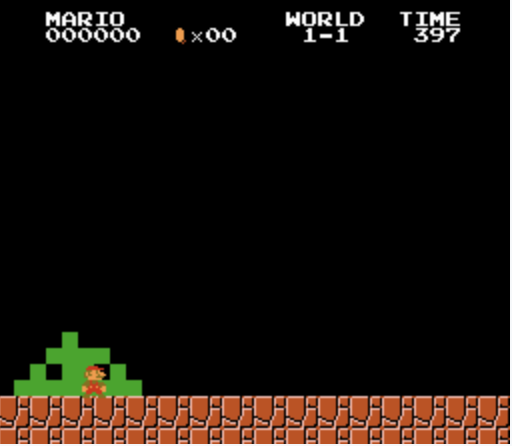
\includegraphics[scale=0.5]{static/mario.png}
  \caption{gym-super-mario-bros游戏界面}
\end{figure}
安装如下:
\begin{lstlisting}[language={bash}]
  pip install gym-super-mario-bros
\end{lstlisting}
使用示例如下:
\cleardoublepage
\begin{lstlisting}[language={python}, caption={super-mario控制}]
from nes_py.wrappers import BinarySpaceToDiscreteSpaceEnv
import gym_super_mario_bros
from gym_super_mario_bros.actions import SIMPLE_MOVEMENT
env = gym_super_mario_bros.make('SuperMarioBros-v0')
env = BinarySpaceToDiscreteSpaceEnv(env, SIMPLE_MOVEMENT)

done = True
for step in range(5000):
    if done:
        state = env.reset()
    state, reward, done, info = env.step(env.action_space.sample())
    env.render()

env.close()
\end{lstlisting}


\section{输入输出}
在游戏的每一个状态(画面像素帧),输入为超级马里奥最近4个画面像素帧的灰度图像。使用最近4个画面是为了让模型学习到当前马里奥的状态(高度,速度,移动方向等等)以及敌人的运动状态。为了使计算机更加容易理解计算机中的画面,使用超级玛丽北京为黑色的环境,这样原本背景的蓝天白云的噪声将不会产生影响。
每一个状态经过现实网络模型的输出为当前超级马里奥可以选择执行的动作,包括上下左右,跳跃,以及这些动作的组合:
\begin{lstlisting}[language={python}]
SIMPLE_MOVEMENT = [
  ['NOOP'],
  ['right'],
  ['right', 'A'],
  ['right', 'B'],
  ['right', 'A', 'B'],
  ['A'],
  ['left'],
]
\end{lstlisting}
\section{Reward以及目标}
本游戏的$reward$有以下公式确定:
\begin{equation}
  reward = V + C + D
\end{equation}
\begin{itemize}
  \item $V$:马里奥上一个状态与当前状态的不同水平位置的差,$V<0$ 代表agent向左走,$V>0$代表agent向右走。
  \item $C$:马里奥上一个状态与当前状态的时间差,代表马里奥在上一个状态到当前状态花了多长时间。
  \item $D$:马里奥是否在上一个状态执行动作后死亡,如果死亡$D=-15$,如果没死$D=0$。
\end{itemize}

$reward$最终会归一化为[-1,1]的范围。

\textbf{本算法控制游戏进行的首要目标为:控制游戏人物每一个回合在没有死亡的情况下,尽可能运动到水平位置距离起点远的位置。}
\section{游戏控制算法}
整个游戏控制算法由DQN算法及其三大改进构成,与传统DQN不同之处在于:
为了减少DQN出现过估计的情况,Q值更新公式采用Double DQN(\ref{alg:double-dqn});
  经验回放时,为了平衡不同样本表现得比率,使网络能够更快的学习到新知识,抽样方法采取Experienced Replay;
  为了使神经网络更深入理解环境本身的价值与动作在环境产生的额外价值,价值神经网络结构采用Dueling-Net的结构。

为了减少画面中原本存在的干扰和加快神经网络的处理速度,会对每一个输入的画面图像有一个预处理过程:
\begin{itemize}
  \item 裁剪掉图像上方对机器来说无意义的信息如分数,生命值,时间值等;
  \item 由于图像较大占用内存过多,因此对其进行缩放为(200*200)的大小;
  \item 将游戏的北京画面改为黑色背景,减少背景产生的干扰。
\end{itemize}

算法描述如算法(\ref{alg:mario})所示:
\begin{algorithm}
  \caption{超级玛丽控制算法}
  \begin{algorithmic}[1]
    \State 初始化Dueling-net网络参数
    \State 初始化经验库memory大小,memory\_size,经验库采用SumTree结构
    \State 初始化游戏,进入状态 s
    \While{经验库没存满}
    \State 随机选择当前状态下能选择的动作a
    \State 执行动作a,到达新的状态s',并获得环境的反馈r
    \State 将状态转化过程<s,a,r,s'>存到经验库memory,更新经验库
    \State 更新状态s $\gets$ s'
    \EndWhile
    \State 设置游戏进行学习的回合总数n
    \State 设置网络更新频率freq
    \State 设置网络的学习频率learning\_freq
    \For{i in range(n)}
    \State 获取当前的状态s
    \State $s_i$作为q-eval网络的输入,得到输出的动作$a_i$
    \State 执行动作$s_i$,到达新的状态$s_{i+1}$,并获得环境的反馈$r_i$
    \State 将状态转化过程$<s_i,a_i,r_i,s_{i+1}>$存到经验库memory,更新经验库 
    \If{i\% freq == 0}
    \State 将q-eval网络的参数更新到q-target网络
    \EndIf
    \If{i \% learning\_freq == 0}
    \State 从经验库中获取优先级最高的经验$<s_j,a_j,r_j,s_{j+1}>$
    \State q-eval网络从经验中$<s_j,a_j,r_j,s_{j+1}>$学习,更新参数
    \EndIf
    \EndFor
  \end{algorithmic}
  \label{alg:mario}
\end{algorithm}
\begin{figure}
  \centering
  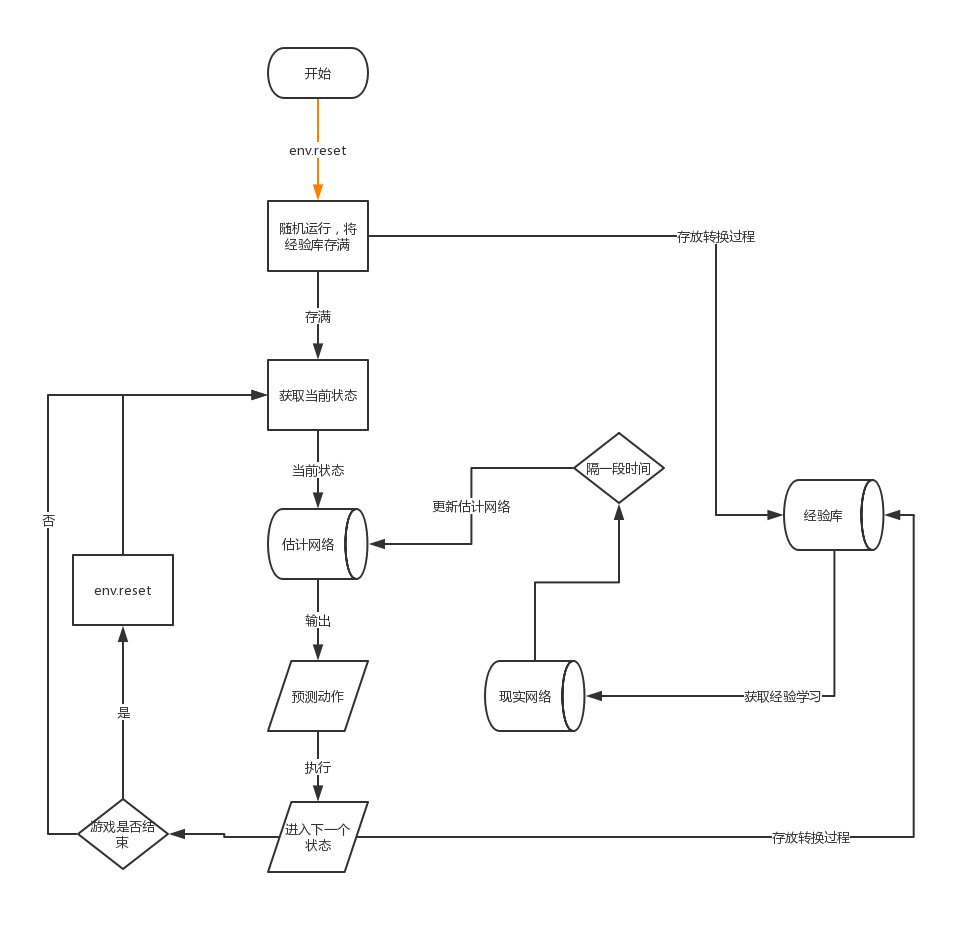
\includegraphics[scale=0.4]{static/graph.png}
  \caption{算法控制过程流程图}
\end{figure}
\cleardoublepage

\section{网络模型结构}

网络结构图如(\ref{fig:net})所示,输入为(32,4,200,200)大小的图片,其中32是batch\_size的大小,经过经过三个卷积层,每个卷积层的激活函数为Relu,然后是池化操作。卷积处理完成之后经过线性连接层分别得到网络输出的动作值以及当前状态的advantage。下面是网络结构每一层从输入到输出的具体结构:
\begin{enumerate}
  \item 输入:输入为(32,4,200,200)大小,其中32是批处理的batch\_size大小
  \item 卷积层:卷积核大小为8,步幅长度为4,经过激励函数为Relu,然后经过池化层,最后单个处理的输出为(32,24,24)
  \item 卷积层:卷积核大小为4,步幅长度大小为2,,经过激励函数Relu,然后进行池化操作,最后单个输出为(64,5,5)
  \item 卷积层:卷积核大小为2,步幅长度大小为2,经过激励函数Relu,然后进行池化操作,最后单个输出为(128,2,2)
  \item 卷积之后连接到两个不同的全连接层:
  \begin{enumerate}
    \item value连接层,输入为2*2*128,中间含有一个大小为128隐藏层,输入为1,即当前环境的价值
    \item advantage连接层,输入为2*2*128,中间含有一个大小为512的隐藏层,输出个数为动作总数,表示每个动作当前的优势值
  \end{enumerate}
  \item 最终输出:$value+(advantage-mean(advantage))$
\end{enumerate}
\begin{figure}
  \centering
  \caption{超级玛丽控制所使用的网络结构}
  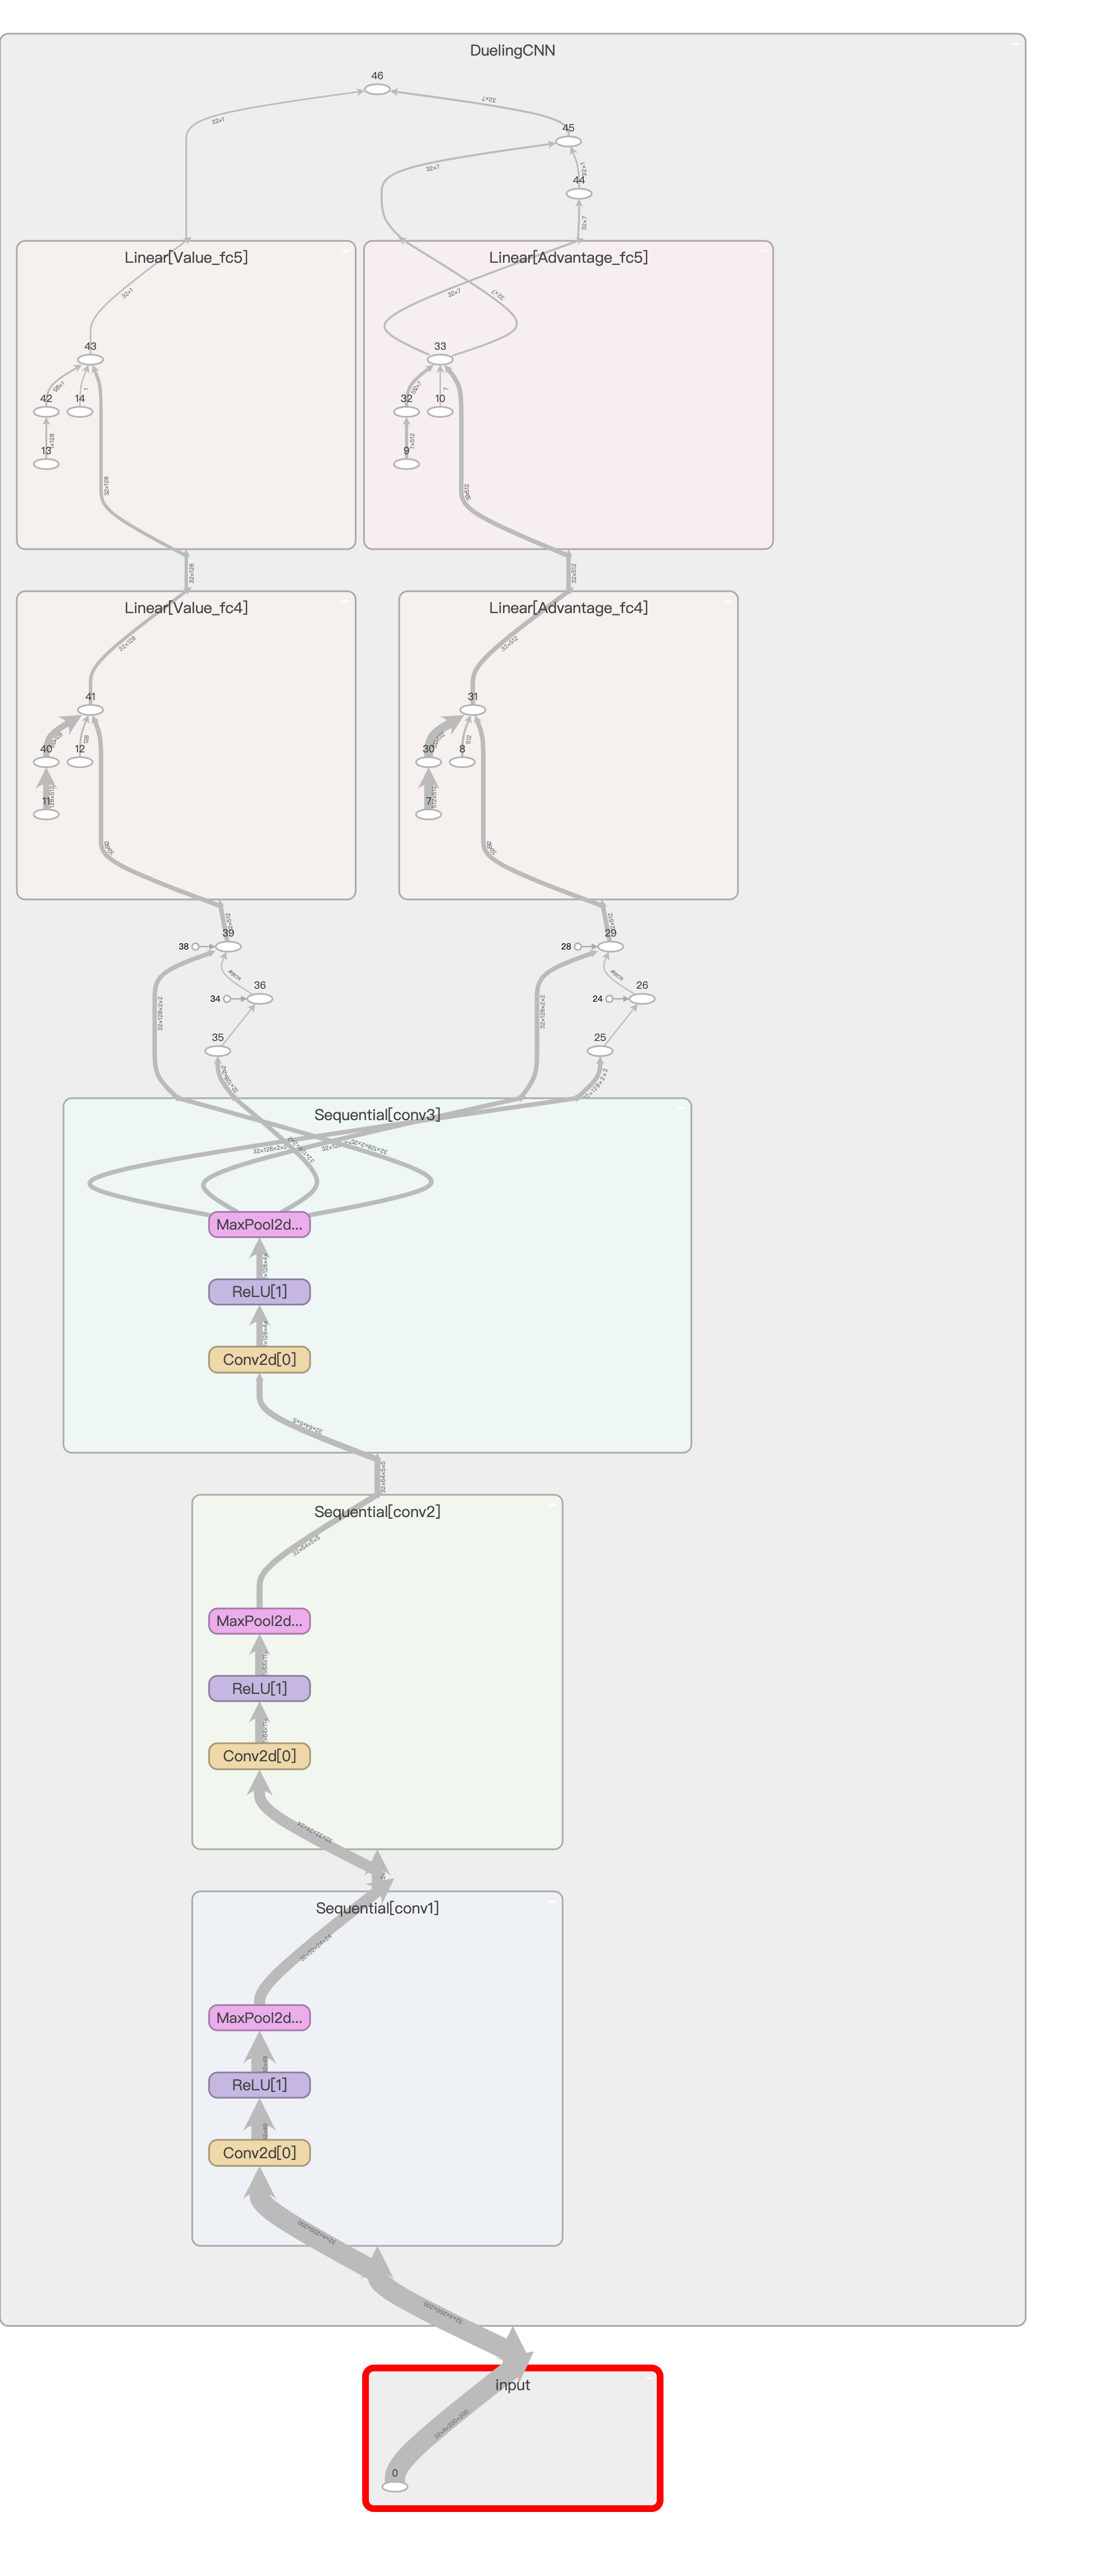
\includegraphics[width=500pt,height=700pt]{static/dueling_net.png}
  \label{fig:net}
\end{figure}
\cleardoublepage
\section{游戏控制的难点}
\begin{figure}[!htp]
  \centering
  \begin{subfigure}{3cm}
      \centering
      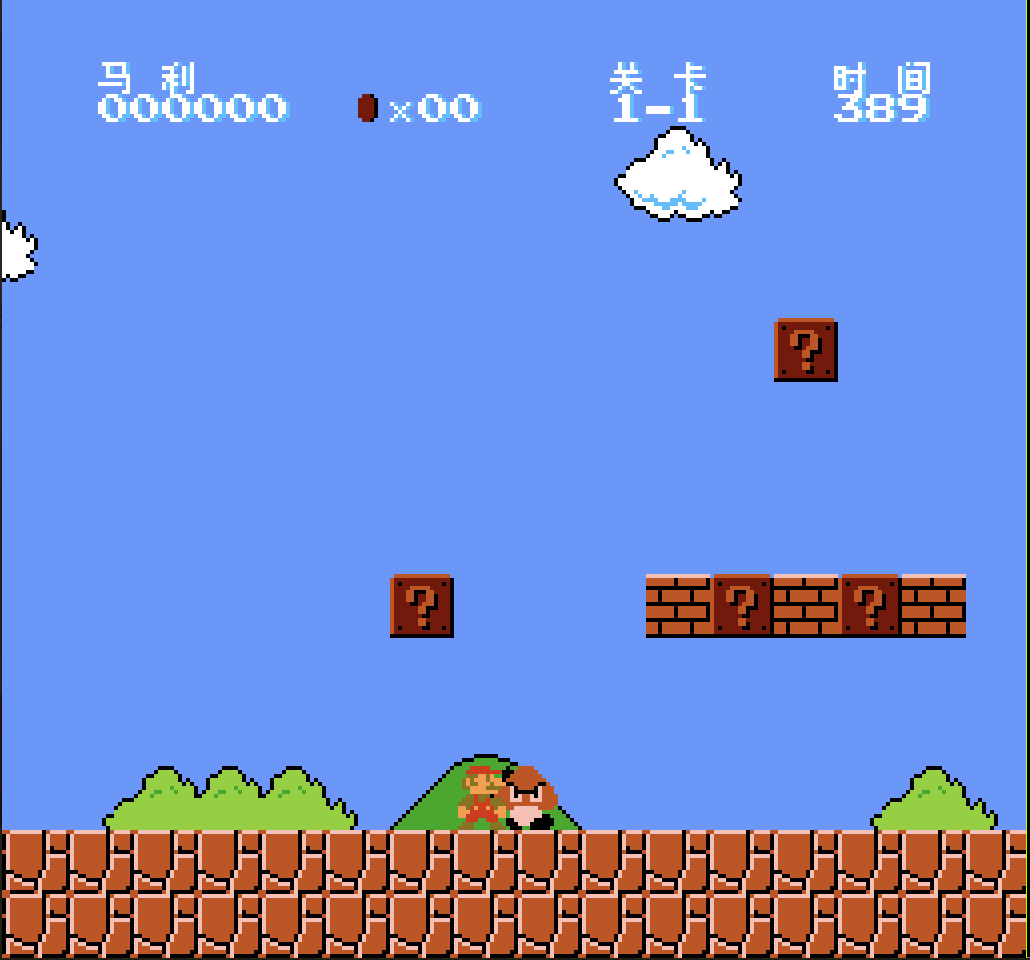
\includegraphics[height=3cm]{static/a.png}
      \caption{遇到第一个NPC}
  \end{subfigure}
  \hspace{1em}
  \begin{subfigure}{3cm}
    \centering
    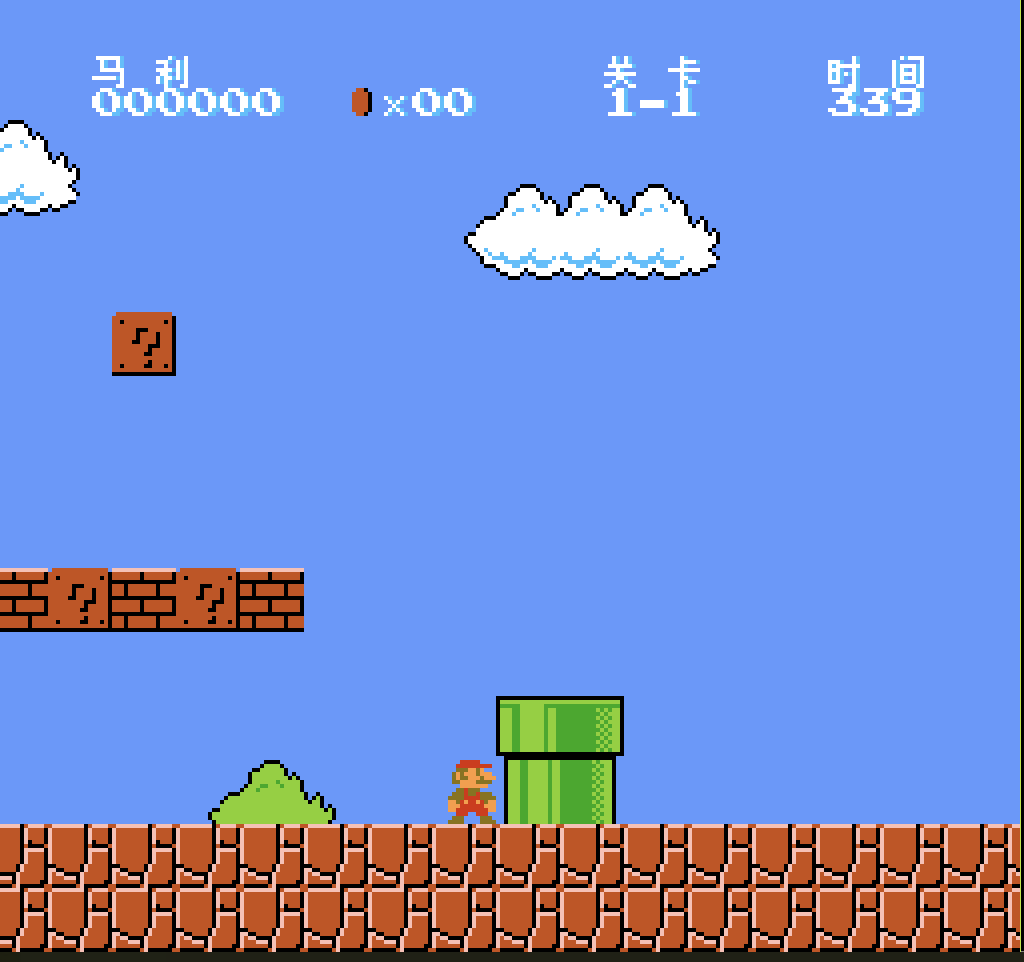
\includegraphics[height=3cm]{static/b.png}
    \caption{遇到第一个水管}
  \end{subfigure}
  \hspace{1em}
  \begin{subfigure}{3cm}
    \centering
    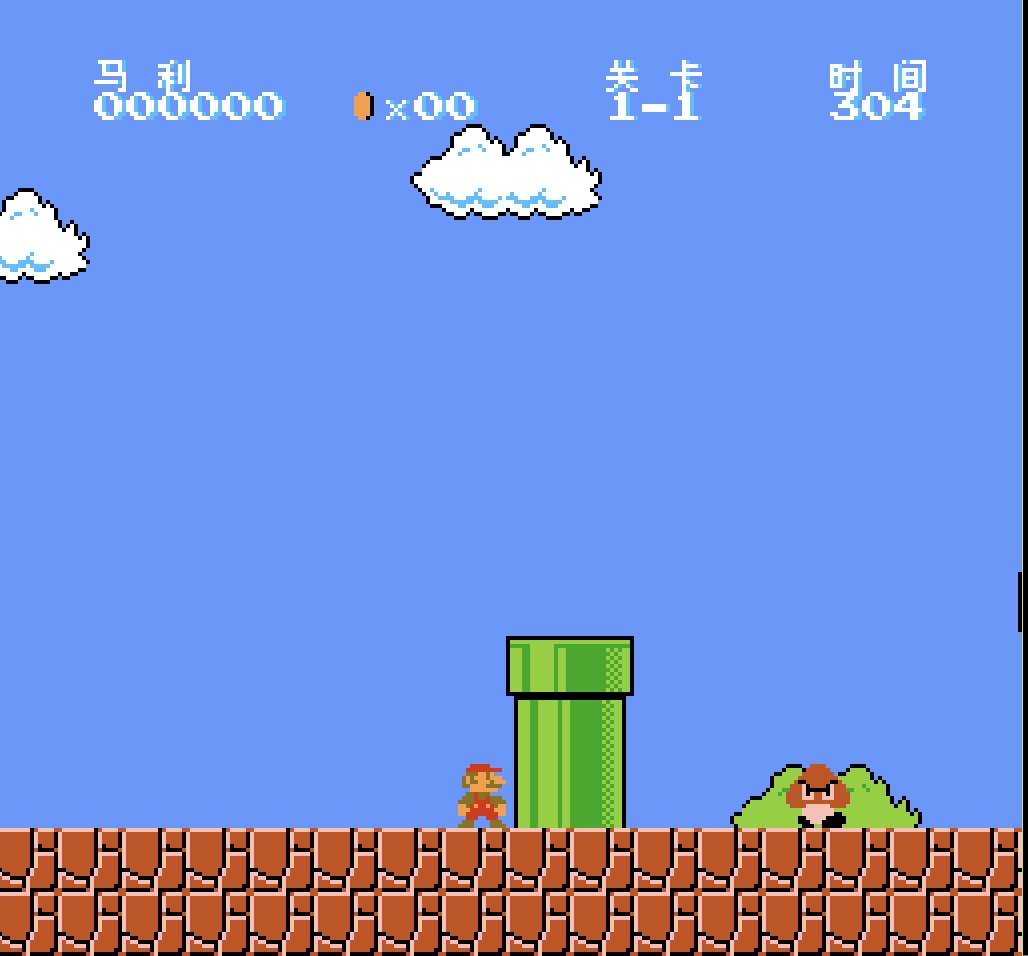
\includegraphics[height=3cm]{static/c.png}
    \caption{遇到比较高的水管}
  \end{subfigure}
  \hspace{1em}
  \begin{subfigure}{3cm}
    \centering
    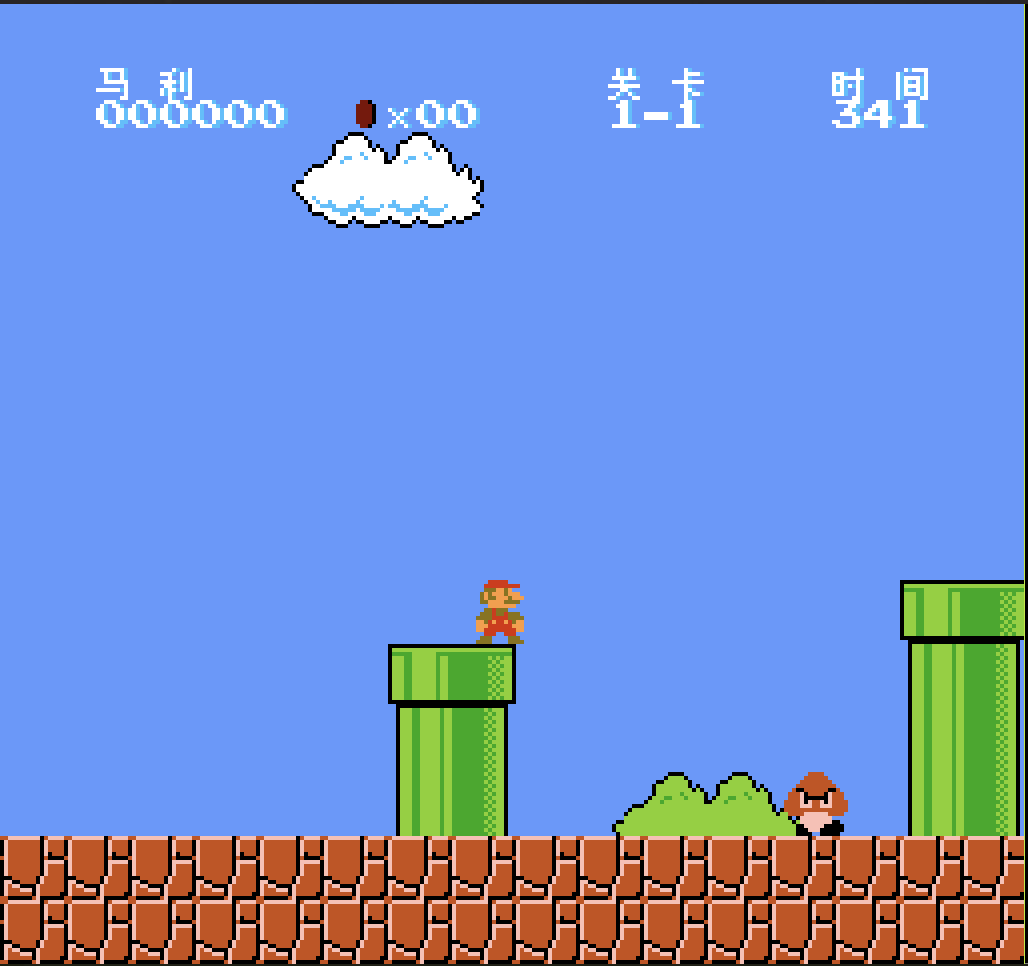
\includegraphics[height=3cm]{static/d.png}
    \caption{跳下水管}
  \end{subfigure}

  \begin{subfigure}{3cm}
      \centering
      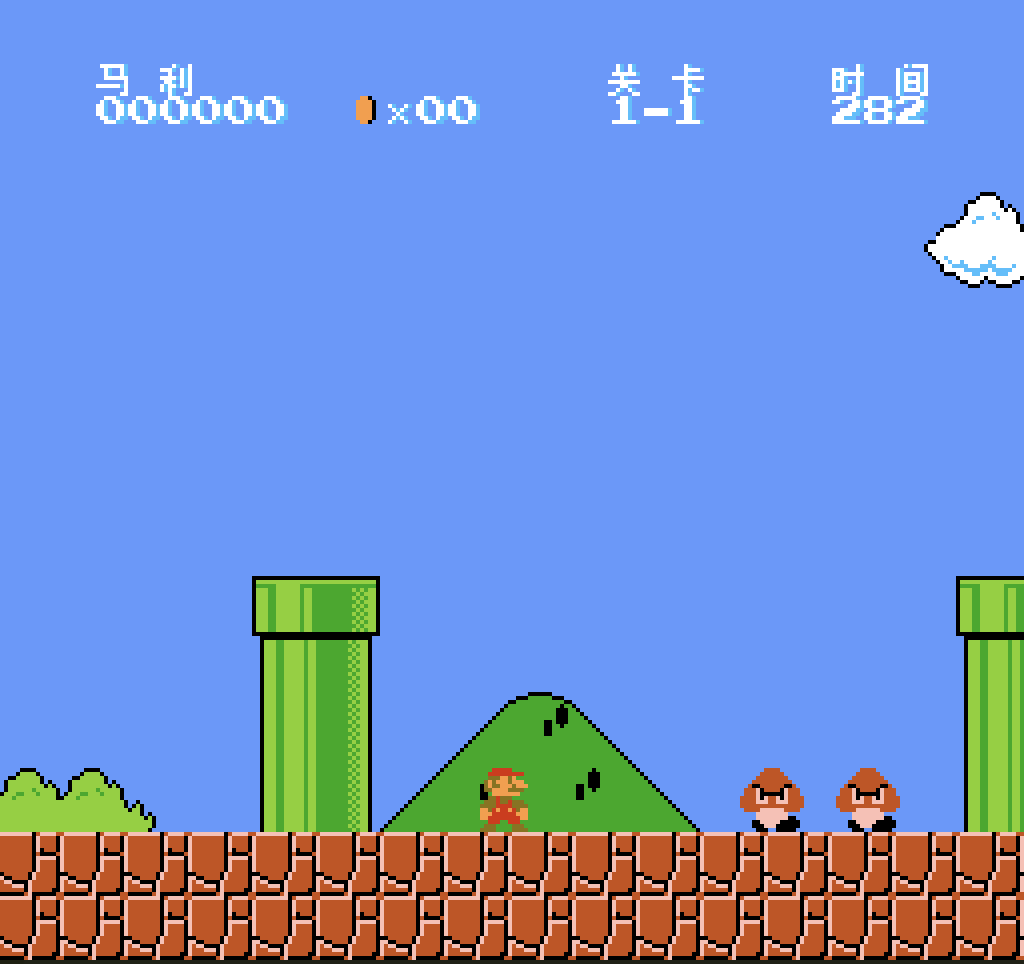
\includegraphics[height=3cm]{static/e.png}
      \caption{遇到最高的水管}
  \end{subfigure}
  \hspace{1em}
  \begin{subfigure}{3cm}
    \centering
    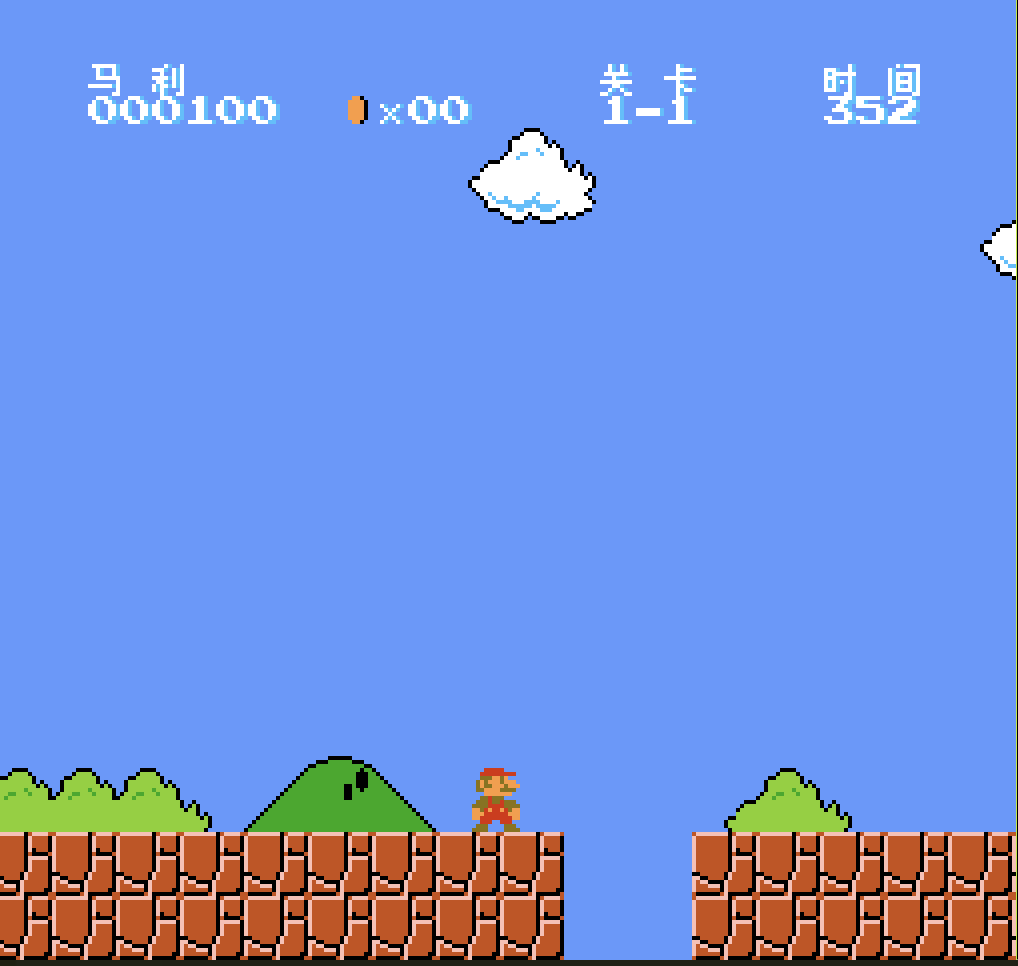
\includegraphics[height=3cm]{static/f.png}
    \caption{遇到第一个坑}
  \end{subfigure}
  \hspace{1em}
  \begin{subfigure}{3cm}
    \centering
    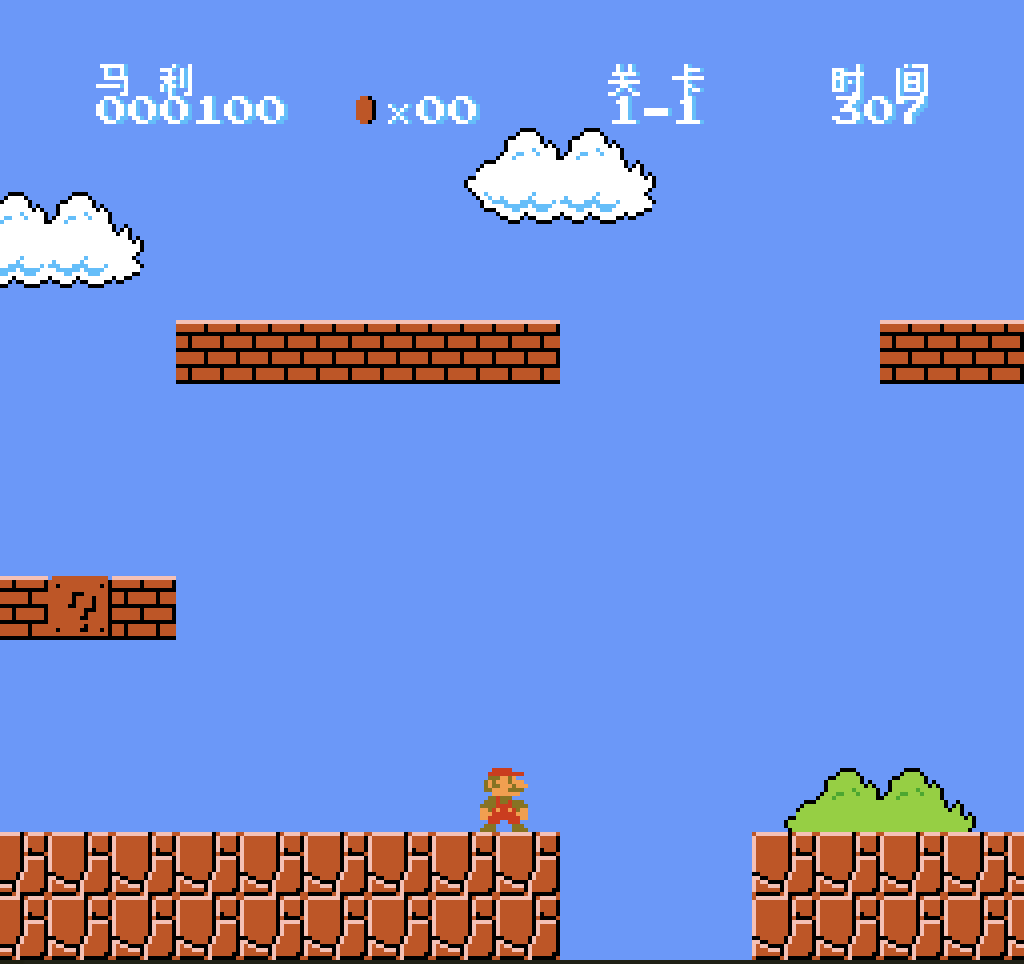
\includegraphics[height=3cm]{static/g.png}
    \caption{遇到第二个坑}
  \end{subfigure}
  \hspace{1em}
  \begin{subfigure}{3cm}
    \centering
    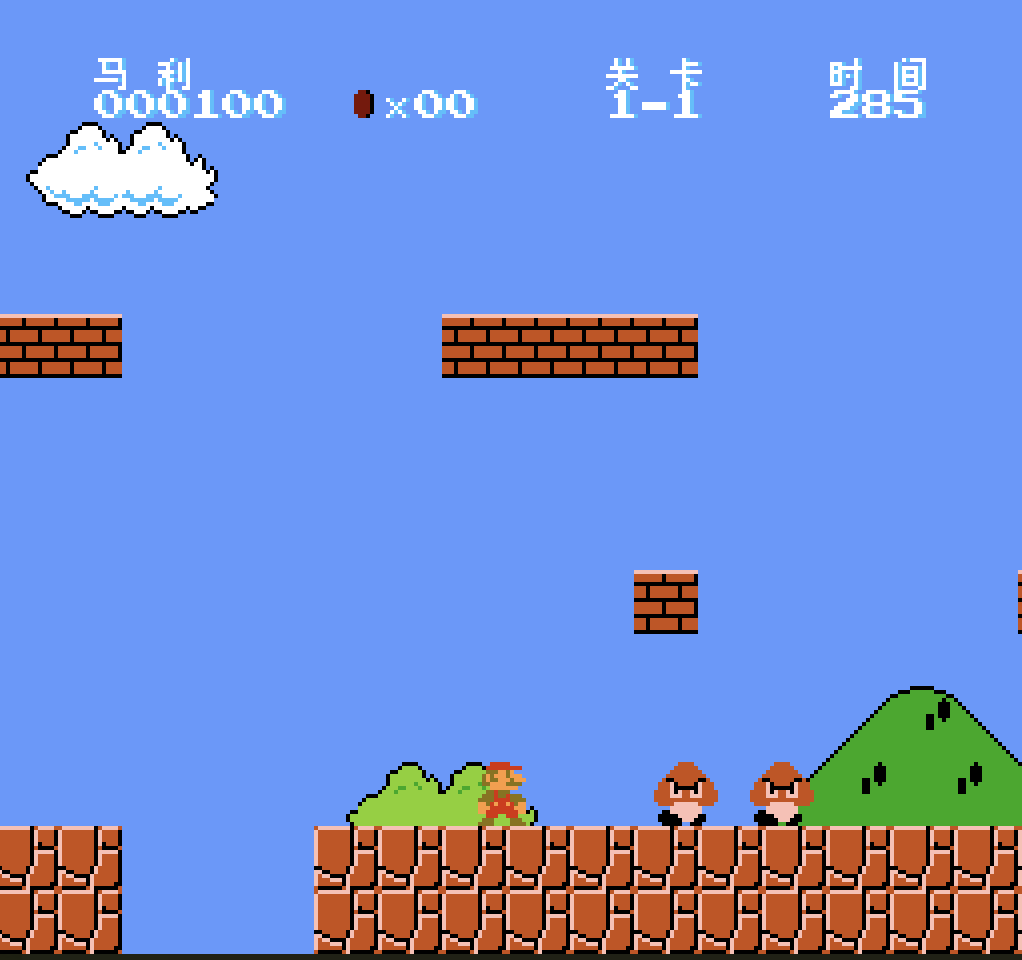
\includegraphics[height=3cm]{static/h.png}
    \caption{跳过坑后遇到NPC}
  \end{subfigure}
  \begin{subfigure}{3cm}
      \centering
      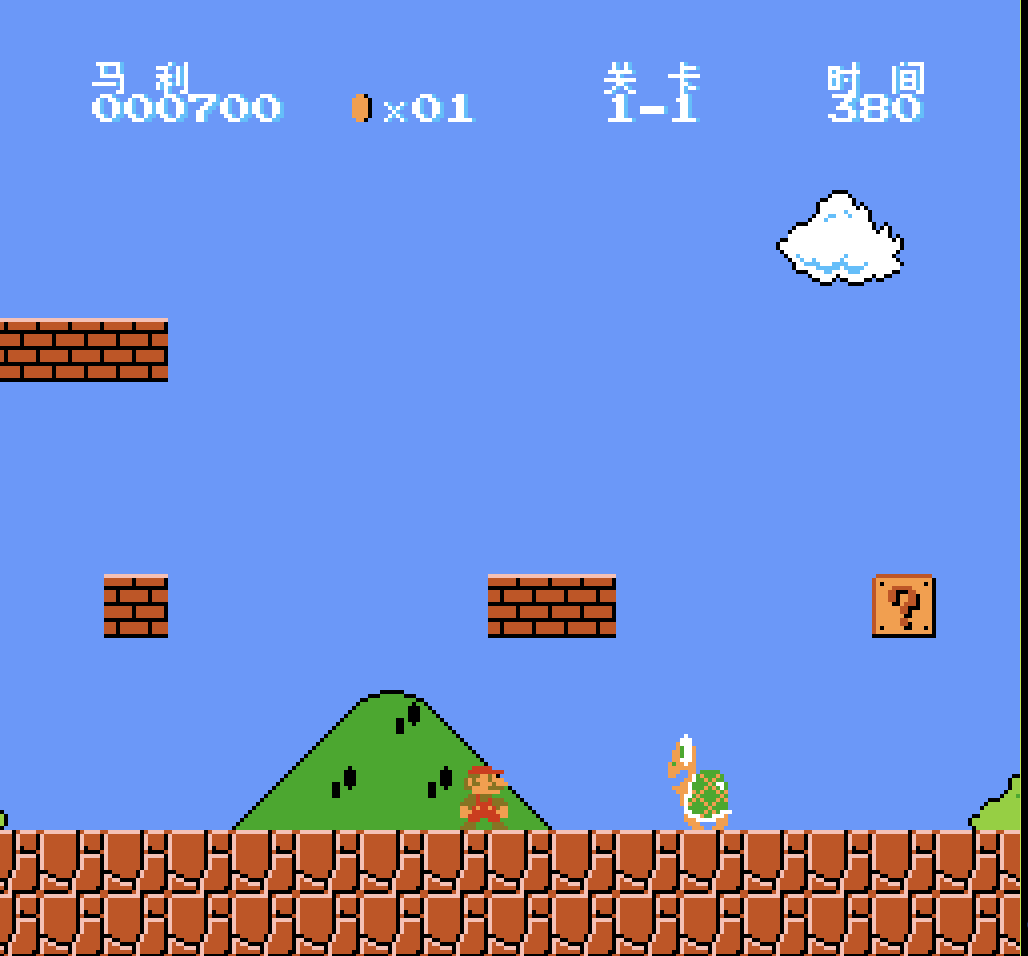
\includegraphics[height=3cm]{static/i.png}
      \caption{跳跃刚结束遇到NPC}
  \end{subfigure}
  \hspace{1em}
  \begin{subfigure}{3cm}
    \centering
    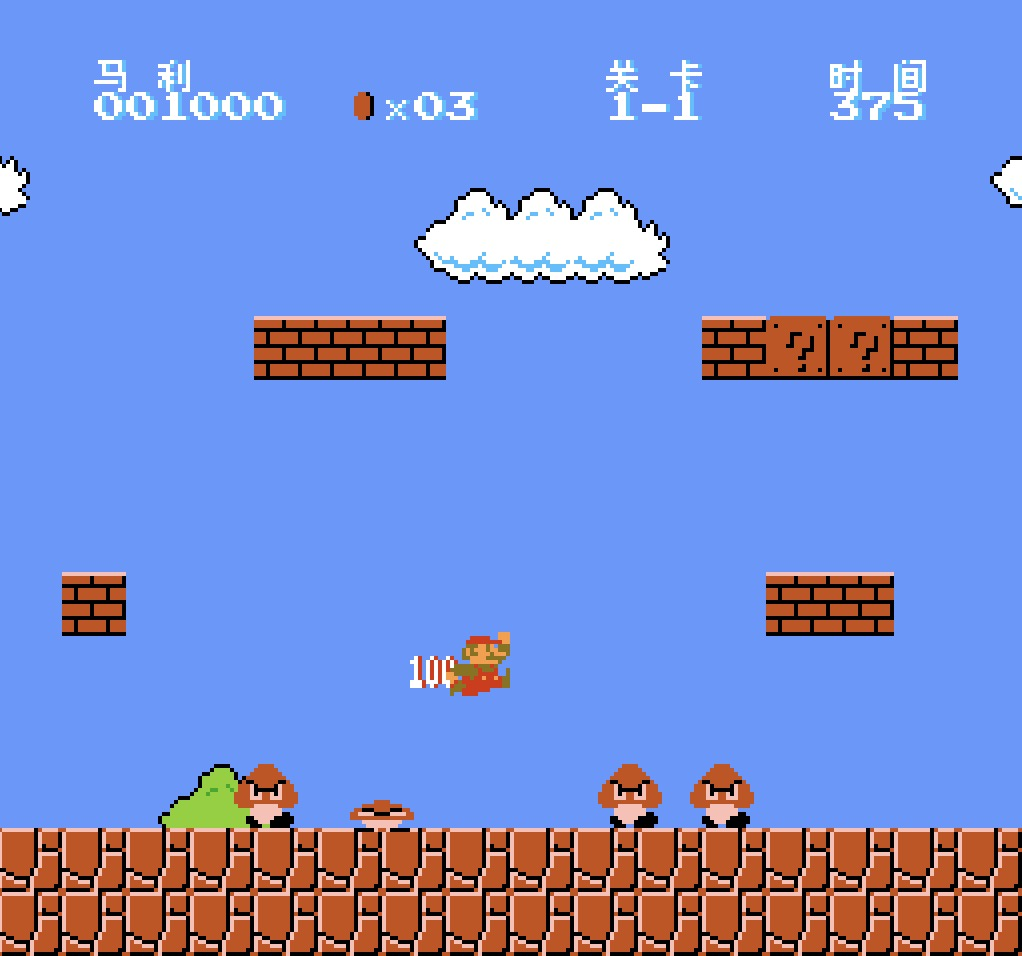
\includegraphics[height=3cm]{static/j.png}
    \caption{最难的点}
  \end{subfigure}
  \hspace{1em}
  \begin{subfigure}{3cm}
    \centering
    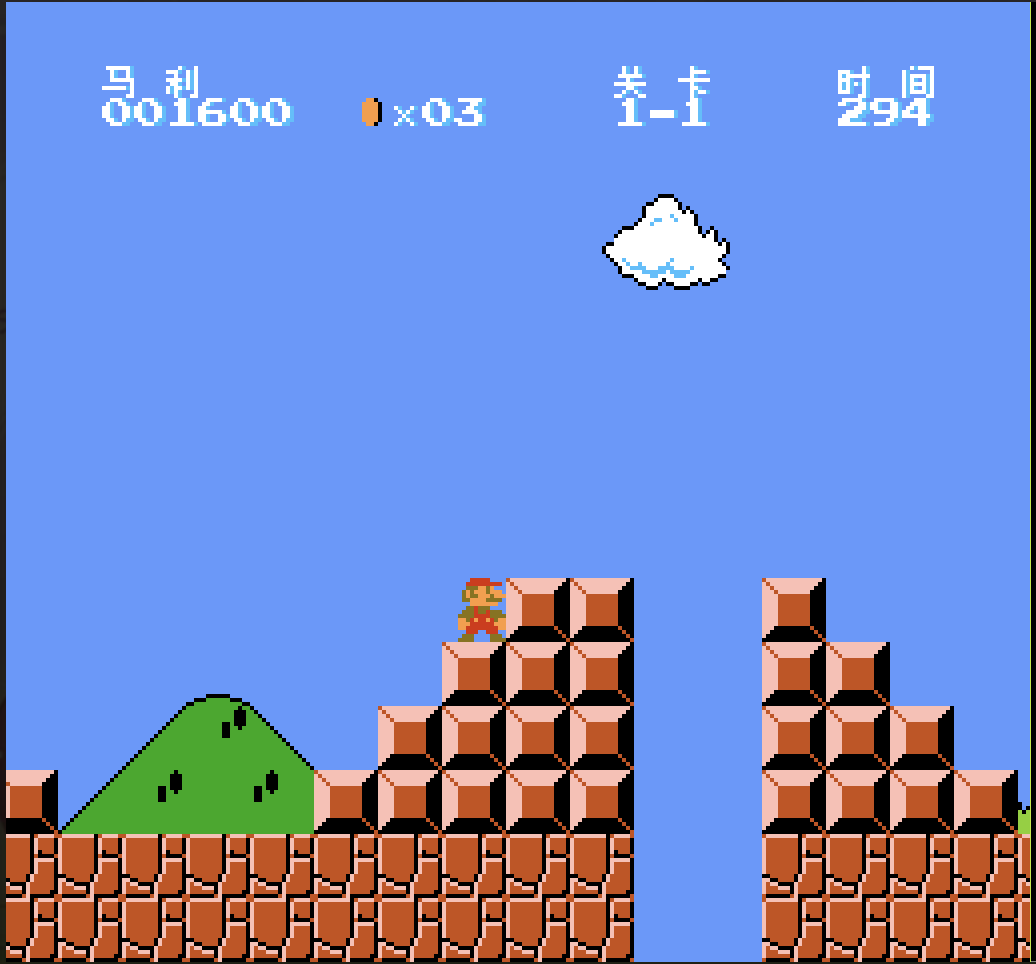
\includegraphics[height=3cm]{static/l.png}
    \caption{最后一个坑}
  \end{subfigure}
  \hspace{1em}
  \begin{subfigure}{3cm}
    \centering
    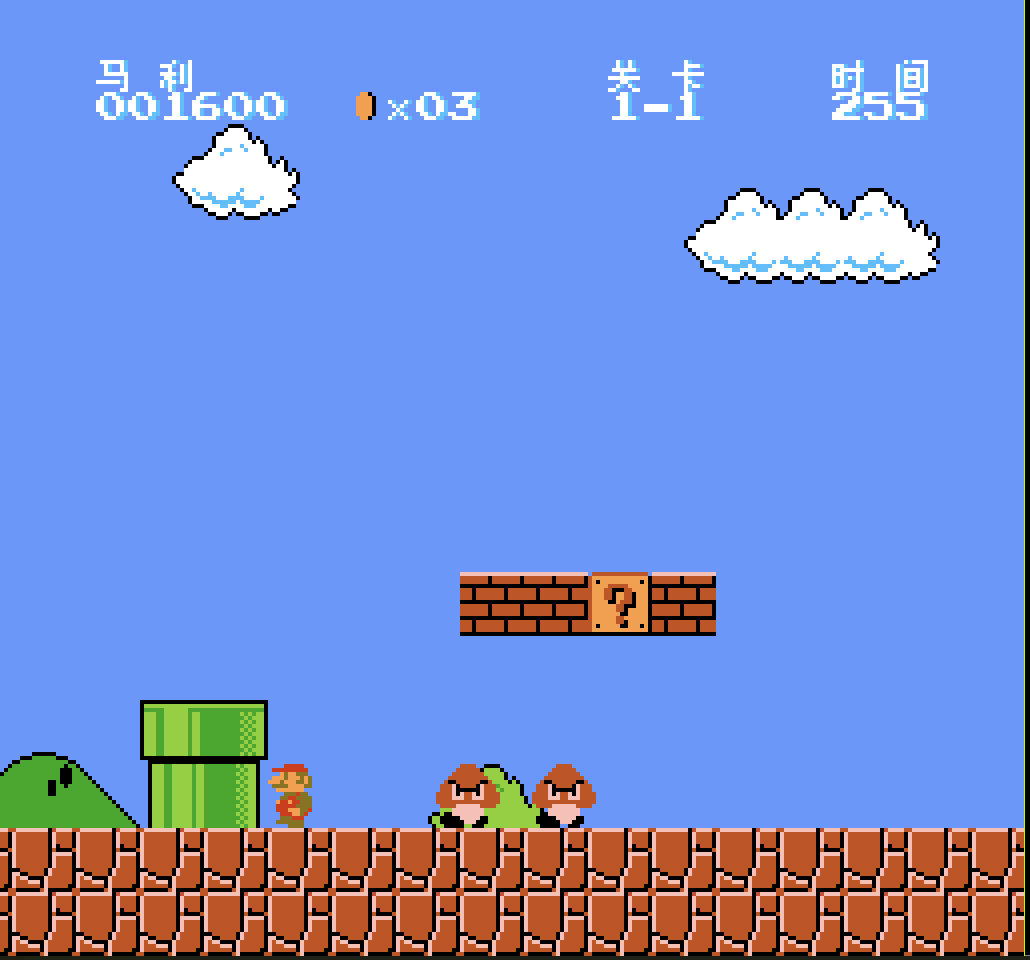
\includegraphics[height=3cm]{static/m.png}
    \caption{最后遇到的NPC}
  \end{subfigure}
  \label{fig:mario}
  \caption{超级玛丽在游戏中的难点}
\end{figure}
\cleardoublepage

由上图游戏的画面,我们可以看到,控制超级玛丽向前运动存在很多处的难点,甚至许多处难点人类来控制也无法做到死亡。在这个游戏当中,对于笔者本身的硬件环境来说,确实很难做到完美。下面是关于这些难点的详细介绍,通过介绍这些难点,可以更加清晰地认识到算法在控制模型做决策时的难易程度:在每个时刻,算法都需要做出以下决策:
\begin{enumerate*}
  \item 当游戏人物处于游戏中任意一个画面时,水平方向选择向左还是向右;
  \item 当游戏人物处于地面上,为了获得更高的奖励,是否需要跳跃;
  \item 如果做出跳跃的决策,应该跳多高(持续多长时间);
  \item 在跳跃的过程中是否做水平移动,向哪个方向做水平移动;
  \item 在跳跃的时候如果移动,应该水平移动多远(持续移动多久)。
\end{enumerate*}
这些决策某个时刻做出,会在不久之后影响后面的状态,有的影响甚至无法挽回。以下将举几个图片的例子来详细说明:
\begin{exmp}[遇到水管]
  在遇到水管的时候,神经网络应该做出决策,决定超级玛丽应该跳多高才能跳过水管,在跳过水管的那一个时刻应该决定向右。
\end{exmp}
\begin{exmp}[跳下水管]
  在跳下水管的时候应该考虑是在什么时机跳下不会遇到NPC而死亡,如果跳的时机不对,刚好遇到NPC,那么这个决策就很失败。
\end{exmp}
\begin{exmp}[遇到深坑]
  遇到深坑的时候,需要决策的更加复杂,坑的宽度不一样,需要跳跃的高度以及跳跃时移动的位置也不一样,如果跳的过早这会掉入坑里,跳的过晚则会直接走到坑里;水平移动的距离太短会导致死亡,水平移动的距离太长则会在落到地上的时刻直接遇到NPC来不及闪躲。
\end{exmp}
\begin{exmp}[遇到NPC]
  在遇到NPC的时候决策是最难的,这个时候需要注意的是可能会遇到不止一个NPC决策,如图j,在遇到NPC需要决定何时跳跃,跳跃落下来的时候会很容易遇到另一个NPC来不及进行第二次跳跃而导致死亡。因此,在实验数据中,在这个位置的动作选择是最难的。
\end{exmp}
